\documentclass[11pt, oneside]{book}

\usepackage{hyperref}
\hypersetup{
    colorlinks=true,
    linkcolor=blue,
    filecolor=magenta,      
    urlcolor=blue,
}
\usepackage{xurl}

\usepackage{adjustbox}
\usepackage{float}
\usepackage{amsmath, amssymb}
\usepackage[inline]{enumitem}
\usepackage{pdfpages}
\usepackage{nameref}

\setcounter{secnumdepth}{4}
\setcounter{tocdepth}{4}

% bar chart
\usepackage{tikz}
\usepackage{pgfplots}
\pgfplotsset{compat=1.16}
\usepgfplotslibrary{statistics}
% ----------------------------------------

\usepackage{xepersian}
\settextfont{Yas}
\setdigitfont{Yas}

\begin{document}
\frontmatter
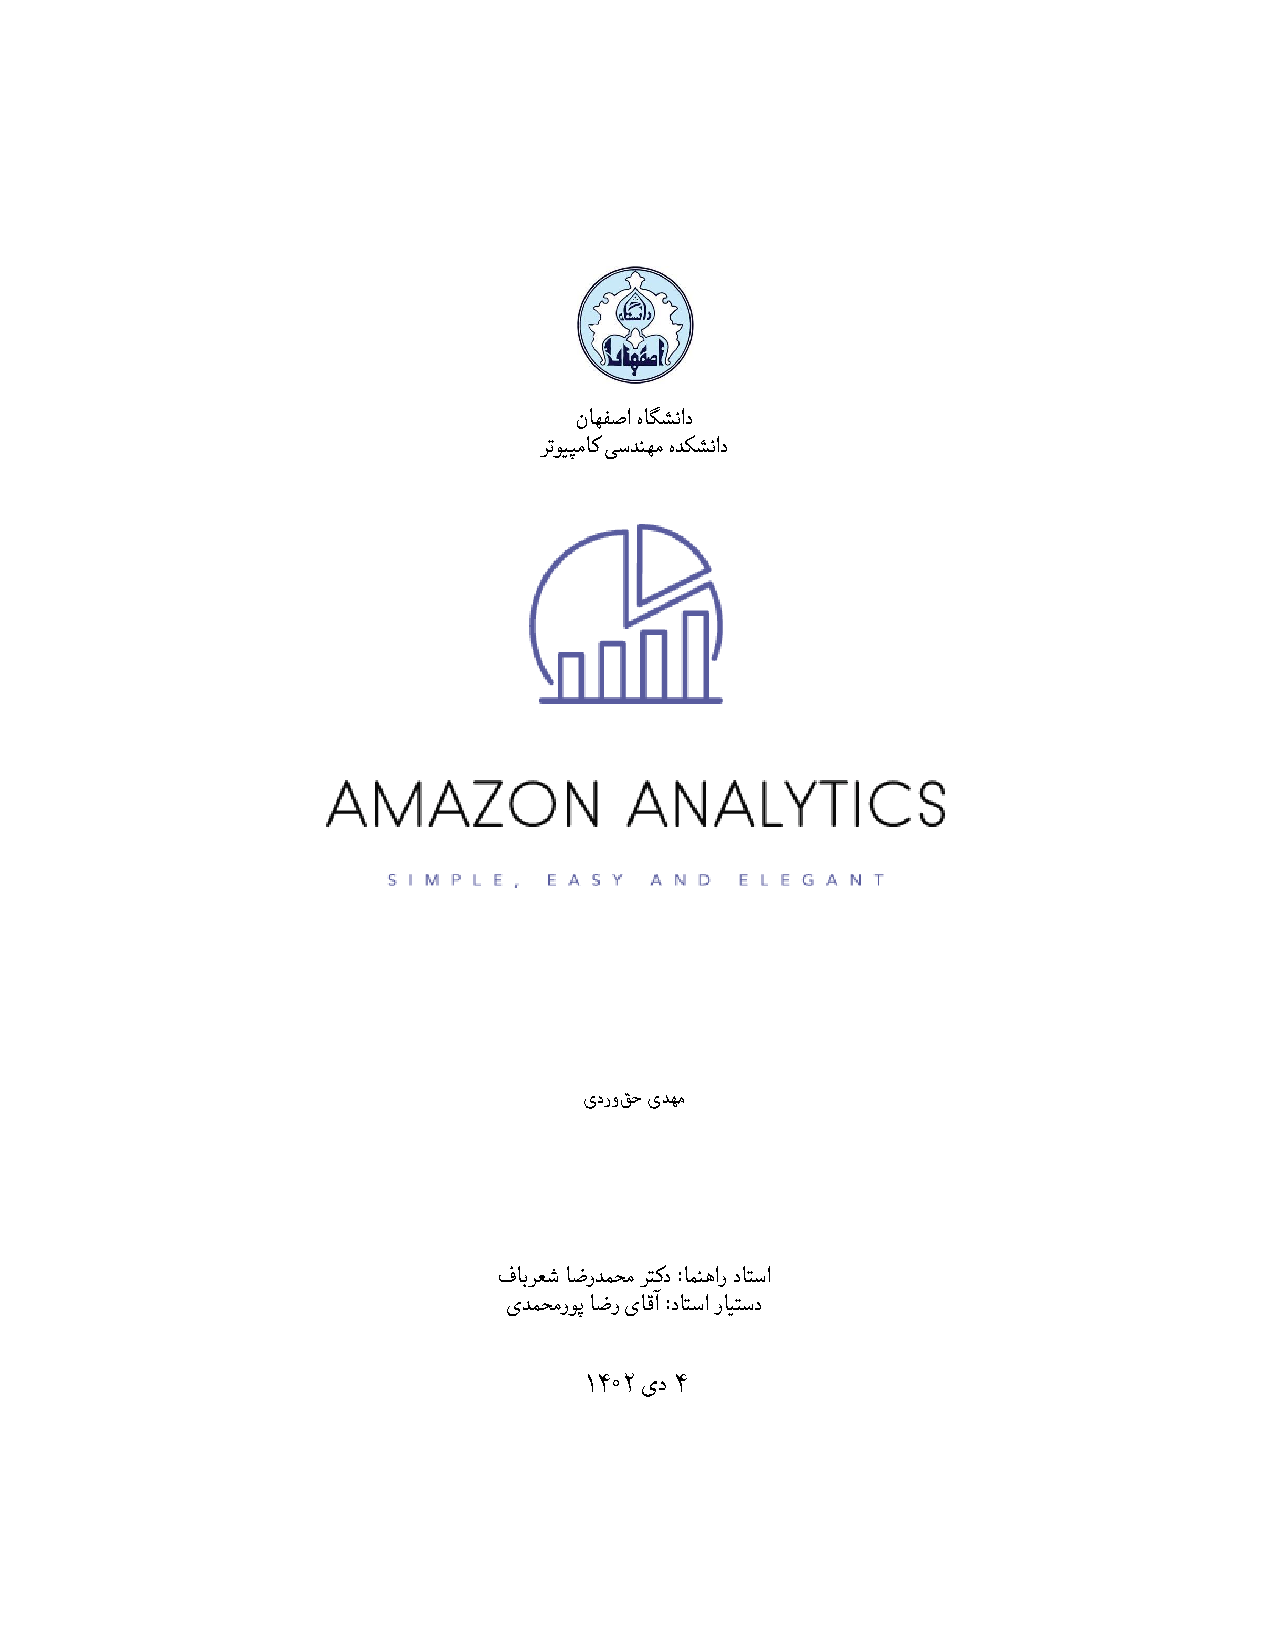
\includepdf{../titlepage/atitle}
\tableofcontents
\mainmatter

\chapter{توضیحات نسخه دمو}
در این فصل به بررسی آنچه که از پروژه‌ی 
\lr{Amazon Analytics}
به صورت دمو پیاده‌سازی می‌شود، پرداخته می‌شود. آنچه که لازم به ذکر است این‌ست که، تمامی مطالعات صورت گرفته برای پروژه‌ی
\lr{Amazon Analytics}
انجام شده، بر اساس پیاده‌سازی از صفر بوده، و همچنین با توجه به فاز سوم پروژه، نیازمند حداقل ۱۳ ماه برای پیاده‌سازی است. به همین جهت، نسخه‌ی دمو تنها قسمت کوچکی از اصل پروژه خواهد بود.

نسخه‌ی دمو قرار است یک وب اپلیکیشن باشد که ۴ قسمت اصلی دارد: 
\begin{enumerate*}
\item 
بخش کاربران،
\item 
بخش 
\lr{Stock}،
\item 
بخش 
\lr{Site}
و
\item
بخش 
\lr{Shipment}. 
\end{enumerate*}
در هر یک از این بخش‌ها، اطلاعاتی که داده‌هایش در پایگاه‌های داده‌ای در سیستم ذخیره‌ هستند، به شکل‌های 
\begin{enumerate*}
\item 
جدول و
\item 
نمودار میله‌ای
\end{enumerate*}
نشان داده می‌شوند.
\section{قسمت‌های نسخه‌ی دمو}
نسخه‌ی دمو قرار است که بر اساس یک سری داده‌ی ذخیره شده، خروجی‌های مختلفی که در پروژه به آنها پرداخته شده بود، را نشان بدهد. در این بخش قسمت‌های مختلف را نام برده و به بررسی خروجی آنها می‌پردازیم.

\subsection{بخش کاربران}\label{ssec:users}
برای بخش کاربران (برای نسخه‌ی دمو) ما آمار برنامه‌نویسیانی که در شرکت آمازون کار می‌کنند را نشان می‌دهیم. فرض شده‌ است که، برنامه‌نویس‌ها هنگام ورود و خروج با کارت یا اثر انگشت، ورود و خروج خود را ثبت کرده‌اند. به علاوه، برنامه‌نویس، \lr{task}هایی که انجام داده‌ است را جایی ثبت کرده و تیک آنها را زده. از طرفی، \lr{task}ها خود سطح بندی‌های 
\begin{enumerate*}
\item 
آسان،
\item 
متوسط و
\item
سخت
\end{enumerate*}
را دارند؛ که به ترتیب ضریب‌‌های $0.5$، ۱ و ۲ را دارند.

متریکی که در این بخش‌ برای برنامه‌نویس‌ها انتخاب شده است، بدین‌گونه محاسبه می‌شود:
\begin{equation}
\frac{
    (\text{تعداد تسک سخت} \times 2) 
    + (\text{تعداد تسک متوسط} \times 1) 
    + (\text{تعداد تسک آسان} \times 0.5)
}{
    \text{ساعات کاری (خروج \ensuremath{-} ورود)}
}
\end{equation}

جدولی به مدیری که مشغول بررسی عملکرد این برنامه‌نویس نشان داده می‌شود، به این صورت است:
\begin{table}[H]
\begin{center}
\caption{جدول \nameref{ssec:users}}
\begin{adjustbox}{width=\textwidth}
\begin{tabular}{|c|c|c|c|c|c|c|c|c|c|}
\hline
نام &
قسمت &
تاریخ &
ورود &
آسان &
متوسط &
سخت &
خروج &
بهروی &
پیشرفت \\
\hline
\hline
مهدی حق‌وردی &
توسعه‌ی \lr{AA} &
\today &
08:00 &
3 &
2 &
4 &
16:00 &
$1.4375$ &
$+0.3$ \\
\hline
حسین هاشمی &
توسعه‌ی \lr{AA} &
\today &
09:00 &
5 &
4 &
5 &
18:00 &
$1.83$ &
$+0.6$ \\
\hline
\end{tabular}
\end{adjustbox}
\end{center}
\end{table}

\subsection{بخش \lr{Stock}}\label{ssec:stock}
برای بخش 
\lr{Stock}
(برای نسخه‌ی دمو) ما فرض کرده‌ایم که به محض اینکه کالایی از سایت، خریداری می‌شود و درخواست پردازش آن به یک انبار می‌رود، زمان درخواست ثبت شده و وقتی از انبار هم خارج می‌شود، باز هم زمان آن ثبت شده و برای سیستم 
\lr{Amazon Analytics}
فرستاده می‌شود.

با چنین داده‌هایی میتوانیم یک متریک به شکل زیر تعریف کنیم:
\begin{equation}
\frac{\text{تعداد کارمند} \times \text{میانگین زمان پردازش}}{\text{تعداد پردازش}} \times 100
\end{equation}
در این متریک، هر چه عدد \textbf{کمتر} باشد، بهروی \textbf{بیشتر} است.

\subsubsection{جدول}
برای این بخش ما چنین جدولی را ارائه می‌دهیم:
\begin{table}[H]
\begin{center}
\caption{جدول \nameref{ssec:stock}}
\begin{adjustbox}{width=\textwidth}
\begin{tabular}{|c|c|c|c|c|c|c|}
\hline
نام انبار &
تاریخ &
تعداد پردازش &
میانگین زمان &
تعداد کارمند &
بهروی &
پیشرفت \\
\hline
\hline
بیرمنگهام &
\today &
1500 &
$4.5$ ساعت &
25 &
$7.5$ &
$+0.45$ \\
\hline
لندن &
\today &
2300 &
2 ساعت &
20 &
$1.7$ &
$-0.56$ \\
\hline
\end{tabular}
\end{adjustbox}
\end{center}
\end{table}

\newpage
\subsubsection{نمودار}
نموداری که در این بخش ارائه می‌شود، نمودار میانگین زمان پردازش هر کالا، در روز است. برای مثال:
\begin{latin}
\begin{center}
\begin{tikzpicture}
\begin{axis}
[
ybar,
title={\rl{میانگین زمان و بهروری}},
symbolic x coords={14 Jan, 15 Jan, 16 Jan, 17 Jan},
legend pos = north west,
axis y line=none,
axis x line=bottom,
nodes near coords,
enlarge x limits=0.2] 
\addplot+ coordinates {(14 Jan, 2) (15 Jan, 2.25) (16 Jan, 1.4) (17 Jan, 2.9)};
\addplot+ coordinates {(14 Jan, 2.5) (15 Jan, 2.8125) (16 Jan, 1.75) (17 Jan, 3.625)};
\legend{\rl{میانگین زمان}, \rl{بهروری}};
\end{axis}
\end{tikzpicture}
\end{center}
\end{latin}

\subsection{بخش \lr{Site}}\label{ssec:site}
برای بخش 
\lr{Site}
ما دو نمودار را ارائه می‌دهیم: 
\begin{enumerate*}
\item 
نمودار 
\lr{Response time} 
و
\item 
نمودار بازخورد‌های مشتریان
\end{enumerate*}
\subsubsection{نمودار \lr{Response time}}
برای 
\lr{Response time}
هم یک نمودار روزانه تولید می‌شود.
\begin{latin}
\begin{center}
\begin{tikzpicture}
\begin{axis}
[
ybar,
title={\rl{\lr{Response time} در دامنه‌ی \lr{UK}}},
symbolic x coords={14Jan, 15 Jan, 16 Jan, 17 Jan, 18 Jan, 19 Jan},
axis x line=bottom,
nodes near coords,
enlarge x limits=0.05] 
\addplot+ coordinates {(14 Jan, 298) (15 Jan, 300) (16 Jan, 312) (17 Jan, 280) (18 Jan, 288) (19 Jan, 305)};
\end{axis}
\end{tikzpicture}
\end{center}
\end{latin}

\subsubsection{نمودار بازخورد‌های مشتریان}
بازخورد‌های مشترین یک دامنه‌ی خاص\RTLfootnote{برای مثال دامنه‌ی مخصوص \lr{UK}} از سایت،‌ جمع‌آوری شده، و پس از تبدیل به عددی بین ۱ تا ۵، از همه‌ی آنها میانگین گرفته شده و به این شکل نشان داده می‌شوند:

\begin{latin}
\begin{center}
\begin{tikzpicture}
\begin{axis}
[
ybar,
title={\rl{بازخورد‌های مشتریان}},
symbolic x coords={UK, India, US, Brazil},
axis x line=bottom,
nodes near coords,
enlarge x limits=0.2] 
\addplot+ coordinates {(UK, 4.2) (India, 4.4) (US, 4.3) (Brazil, 4.1)};
\end{axis}
\end{tikzpicture}
\end{center}
\end{latin}

\subsection{بخش \lr{Shipment}}\label{ssec:shipment}
در بخش 
\lr{Shipment}
با توجه به اطلاعاتی که در جدول 
\ref{tab:shipment}
ارائه می‌دهیم، چنین متریکی در نظر گرفته‌ایم:
\begin{equation}
\frac{\text{مسافت کل طی شده}}{\text{تعداد کالا} \times \text{میانگین زمان ارسال}} \times 100
\end{equation}

جدول ارائه شده:
\begin{table}[H]
\begin{center}
\caption{جدول \nameref{ssec:shipment}}
\label{tab:shipment}
\begin{adjustbox}{width=\textwidth}
\begin{tabular}{|c|c|c|c|c|c|c|}
\hline
نمایندگی ارسال &
مسافت کل &
تعداد کالا &
میانگین زمان &
تعداد کارمند &
بهروری &
پیشرفت \\
\hline
\hline
\lr{Amazon Post} &
550000 کیلومتر &
1500000 &
3 روز &
20 &
$1.83$ &
$+0.5$ \\
\hline
\lr{UK National Post} &
400000 کیلومتر &
800000 &
2 روز &
18 &
$2.7$ &
$+0.1$ \\
\hline
\end{tabular}
\end{adjustbox}
\end{center}
\end{table}
\end{document}